\section{Experiment Result}
In this section, we will analyze the performance of our algorithm compared to other SVD implementations on CPU and GPU.
In addition, we will discuss the GPU kernel profiling result to show how to improve our implementations.
We also show our performance on huge matrix size.

We tested our algorithm on GeForce 750 Ti, Quadro 600 and Tesla K40c.
The specifications are in Table \ref{tab:spec}.
\begin{table}[h]
\caption{Specifications of Different GPUs}
\centering
\begin{tabular}{|c|c|c|c|}
\hline
Specifications & GeForce 750 & Quandro 600 & Tesla K40 \\ \hline
Architecture   &     Maxwell &       Fermi &    Kepler \\ \hline
CUDA Cores     &         640 &          96 &      2880 \\ \hline
GPU Clock      &    1268 MHz &    1280 MHz &   745 MHz \\ \hline
Mem Size       &        2 GB &        1 GB &     12 GB \\ \hline
Mem Bandwidth  &   86.4 GB/s &   25.6 GB/s &  288 GB/s \\ \hline
\end{tabular}
\label{tab:spec}
\end{table}

\subsection{Comparision to other implementations}
We generated random bidiagonal matrices with double precision numbers in the range of 0 to 1.
In order to obtain relative accuracy experimental results, we generates 10 random matrices.
For each matrix, the SVD algorithm was executed 10 times on GPU.
The average performance does not vary much when more matrices and more times are used.

We compare our algorithm with CULA GPU library, Intel MKL library, Sheetal's QR implementation on S1070, and Liu's divide-and-conquer implementation on M2070.
We measure the performance of CULA on Tesla K40c, and that of Intel MKL on an 8-core cpu with 16 threads.
Until now, CULA library only has QR routine culaDbdsqr.
Intel MKL library has both divide-and-conquer DBDSDC and QR routine DBDSQR.
Usually, divide-and-conquer routine is faster than QR routine, so we select DBDSDC instead of DBDSQR.
We measure the performance of CULA on Tesla K40c, and that of Intel MKL on an 8-core cpu with 16 threads.
For Sheetal's implementation, we use the experimental results of diagonalization listed in the table of their papers.
The results of Liu's are estimated comprehensively according to the figures presented in their paper.

\begin{figure}[hbpt]
\centering
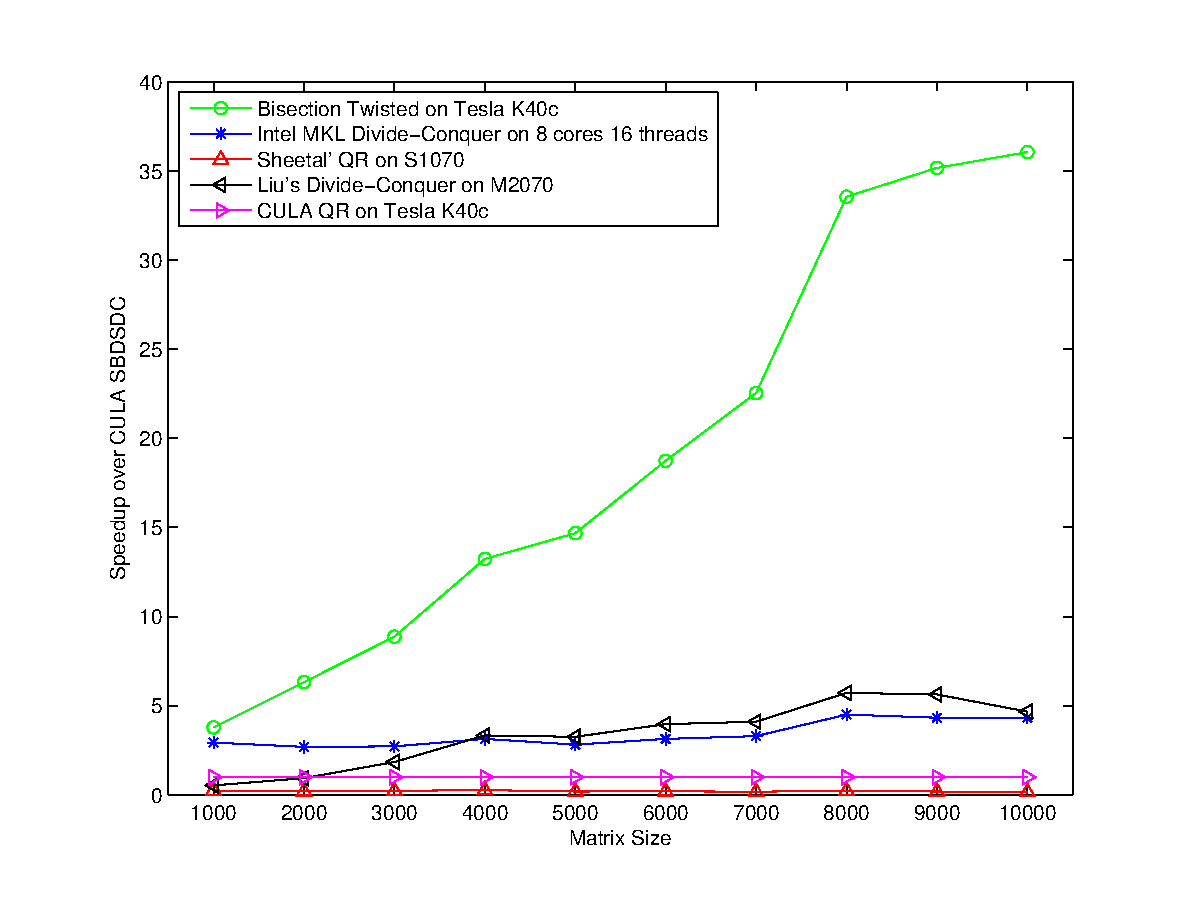
\includegraphics[width=0.5\textwidth]{svd_speedup}
\caption{Overall Performance Comparision}
\label{fig:svd_speedup}
\end{figure}
Figure \ref{fig:svd_speedup} shows the performance of our implementation on Tesla K40c GPU to other existing libraries and implementations.
We selects CULA QR routine BDBSQR as a baseline.
From the figure, we achieve a speedup of 3.8 to 36 over CULA culaDbdsqr routine,
while Intel MKL DBDSDC routine has a 2.9 to 4.3 speedup on a 8 core cpu, and Liu's implementation has only 0.5 to 4.7 speedup over CULA library.
Sheetal's implementation is about 3 to 5.3 times slower than CULA library.
The performance goes up when matrix size becomes large.
Overall, we achieve a speedup of 1.3 to 8.3 over the Intel MKL Divide-Conquer Implementation on CPU, 4 to 7.2 over the Liu's Divide-conquer method, 15 to 288 over the QR implementation Sheetal Paper.

\subsection{Profiling Data}

\subsubsection{the Optimal Block Size}
In our length division design on singular value, the number of block size determines the execution time of the whole singular values.
An inappropriate block division will affect the performance on GPU heavily.
To obtain the optimal block size, we make use of experimental method. 

\begin{figure}[hbpt]
\centering
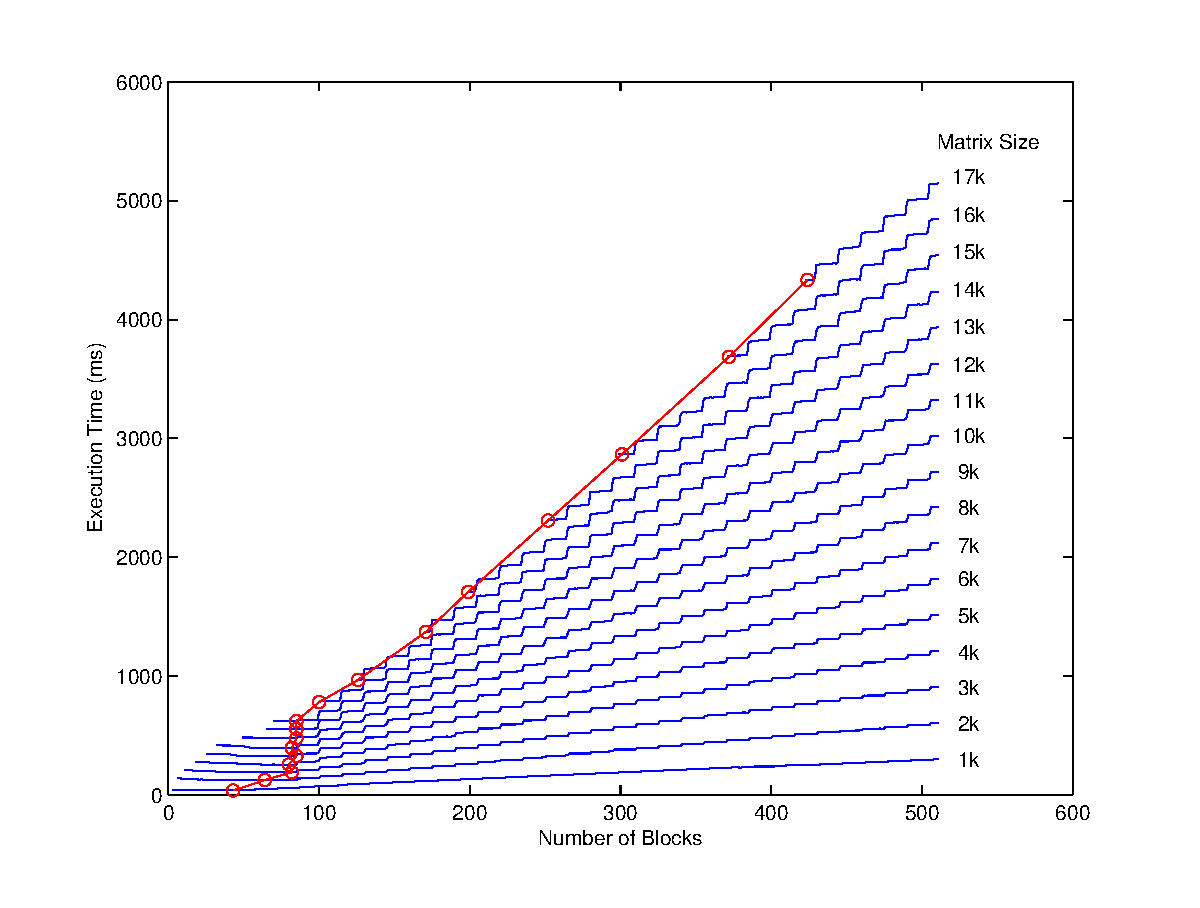
\includegraphics[width=0.5\textwidth]{length_block_num}
\caption{The optimal block number of different matrix size with double precision on Tesla K40c}
\label{fig:length_block_num}
\end{figure}
Figure \ref{fig:length_block_num} shows the elasped time of obtaining all the singular values with different number of blocks and different matrix size on GPU Tesla K40c with double precision.
The blue wavy curves show the relationship between the execution time and the number of blocks on the matrix size in the right column.
From the curves, we can see that the performance goes down slightly first, and then rises when the number of blocks increases.
The left point of the wavy curve shows the minimal number of blocks should be allocated when the matrix size is identified.
In other words, the number of blocks should not be less than the left point on the wavy curves.
When matrix size becomes large, the left point in wave curve trends to a large number of blocks.

The red circle curve in the figure shows the optimal number of blocks with minimal execution time on different size.
we can see that the optimal number of blocks increases when matrix size is less than $3k$,
keeps stable when matrix size is in the range of $3k$ to $9k$,
and becomes the minimal number of blocks when matrix size is lager than $9K$.
Actually, when the block number is close to the optimal number, the execution time does not change too much.
Due to the uncertainty of the input matrix, the optimal block number may vary slightly.
Thus, it is not necessary to select the exact optimal block number.
But it is better to select the number of blocks around the optimal one.

\begin{figure}[hbpt]
\centering
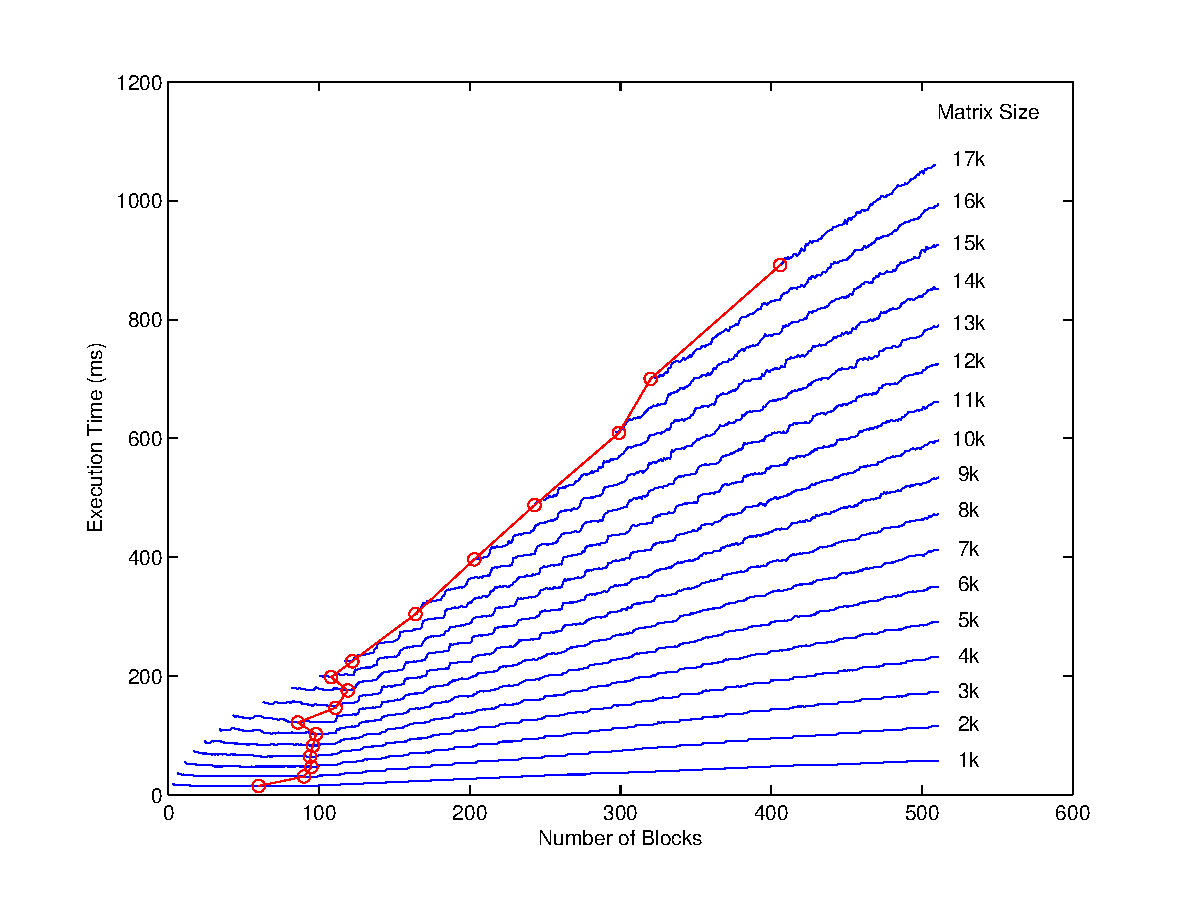
\includegraphics[width=0.5\textwidth]{length_block_single}
\caption{The optimal block number of different matrix size with single precision on GeForce 750 Ti}
\label{fig:length_block_single}
\end{figure}
Figure \ref{fig:length_block_single} is another experimental results on GeForce 750 Ti GPU with single precision.
The curves are very similar with the curves in Figure \ref{fig:length_block_num}.
However, the optimal number of blocks shifts right to be a large number because GeForce has a better architecture than Tesla.
%The reason of the optimal number of blocks is determined by the CUDA cores.
%The Tesla K40c has 15 multiprocessors (MP) and 192 CUDA cores per MP.
%Thus, the total CUDA cores are $2880$ in Tesla K40.
%The GPU code is actually executed in groups of 32 threads called a warp concurrently.

%The optimal GPU block size is not the less, the better.
%It depends on the number of singular values in the subintervals.
%If one have more, GPU will have to wait.
%If all subintervals have the number of singular deviate from the integer multiples of a warp. The GPU efficiency will be less.

\subsubsection{Comparasion of two different Singular Value Design}
In this part, we compare the execution time on two different singular value kernels.
For the length division design, we selects the minimal execution time corresponding to red point curve in figure \ref{fig:length_block_num}.
For the number division design, we selects the minimal number of blocks that is able to allocated, since the execution time does not vary much between the minimal number of blocks and the optimal nubmer of blocks.

\begin{figure}[hbpt]
\centering
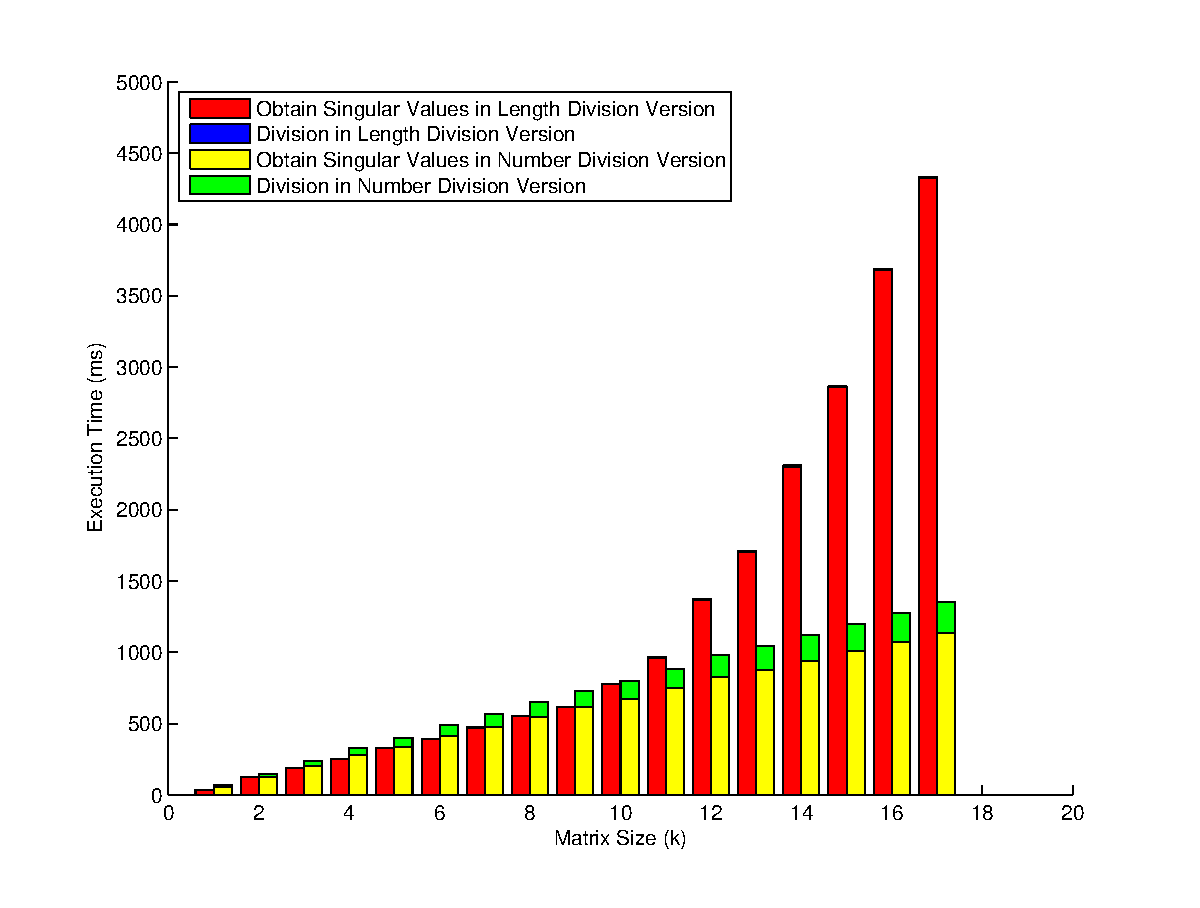
\includegraphics[width=0.5\textwidth]{compare_value_kernel}
\caption{The optimal block number of different matrix size with single precision on GeForce 750 Ti}
\label{fig:compare_value_kernel}
\end{figure}
Figure \ref{fig:compare_value_kernel} shows the execution time of obtaining all singular values of two different implementations on GPU.
The left bar is the execution time of length division design, while the right bar is that of number division design.
From the figure, we can see that when matrix size is less than $9k$, length division version run a little faster than number division version.
When matrix size is larger than $9k$, the execution time of length division version rises quickly, while the execution time of number division version only rises linearly.
Thus, when matrix size becomes larger than $9k$, it is better to select number division kernel.

Also, figure \ref{fig:compare_value_kernel} represents the average execution time on each GPU kernels of two different designs.
When matrix size is smaller than $9k$, the difference between two designs is only on the interval division method.
The division time in length division version is negligible since it is two small, while the division time in number division version increases.
The execution time on obtaining singular values in both version are almost the same when matrix size is less than $9k$.

\subsubsection{Profiling Analysis on Different GPUs}
\textbf{I want to analyze the bound}

\begin{figure}[hbpt]
\centering
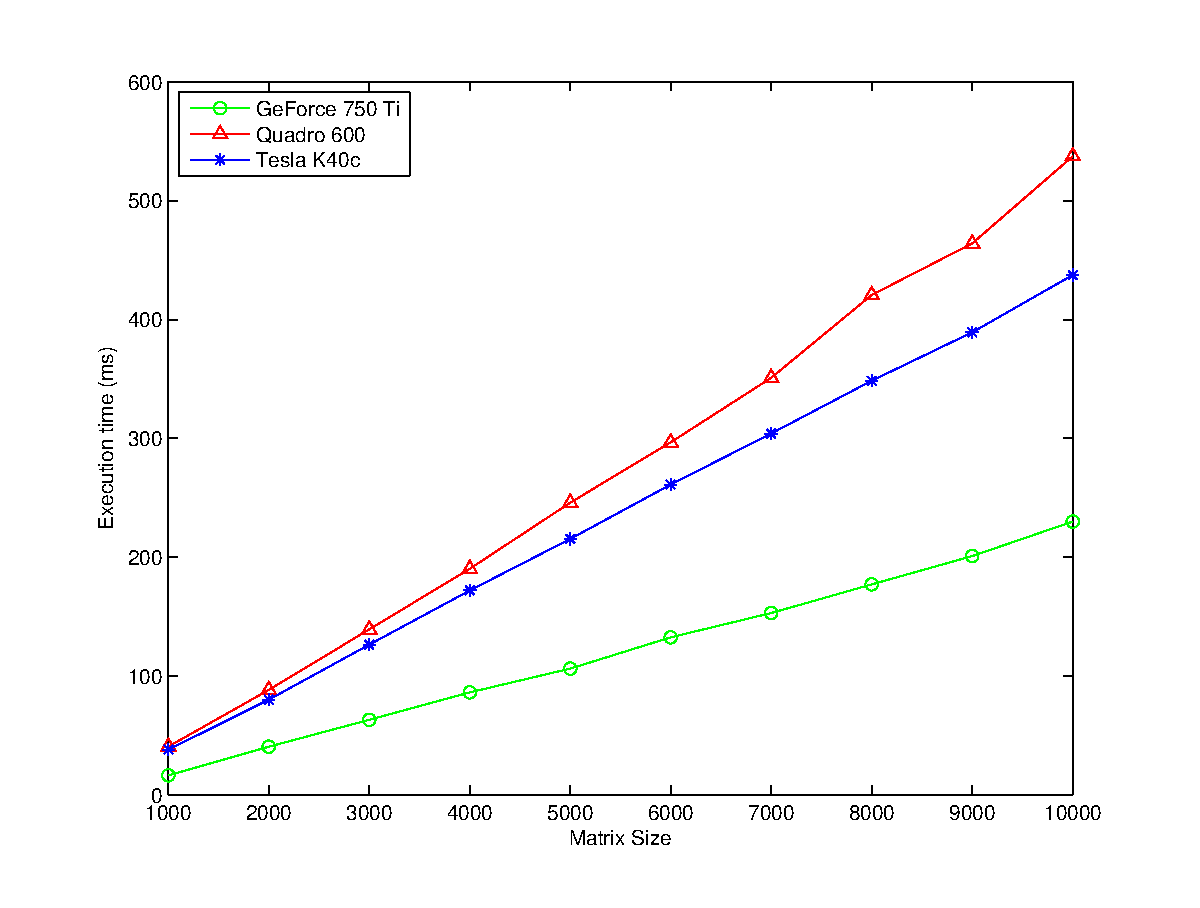
\includegraphics[width=0.5\textwidth]{svd_val_gpus}
\caption{Execution time of number-division singular value kernel on different GPUs with single-float precision}
\label{fig:svd_val}
\end{figure}
Figure \ref{fig:svd_val} shows the execution time of singular value kernel on different GPUs. 

\begin{figure}[hbpt]
\centering
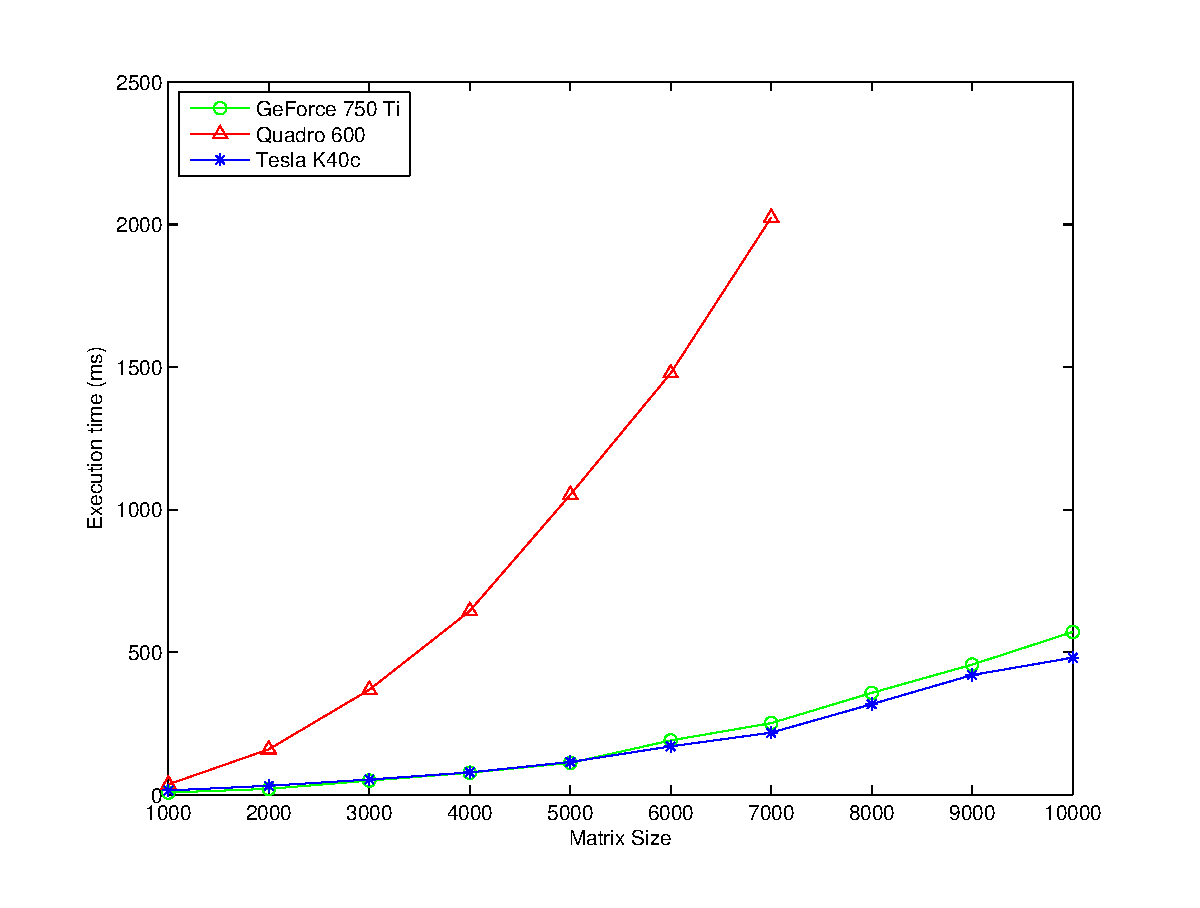
\includegraphics[width=0.5\textwidth]{svd_vec_gpus}
\caption{Execution time of singular value kernel on different GPUs with single-float precision}
\label{fig:svd_vec}
\end{figure}
Figure \ref{fig:svd_vec} shows the execution time of singular vector kernel on different GPUs. 

\subsubsection{Tolerance in Bisection Algorithm}
Since the bisection algorithm is an approximate algorithm to calculate the singular values, we should test the effect of different error tolerance.
The error tolerance $err$ means that the error between the singular values of our algorithm and the actual singular values are less than $err$.
It determines the accuracy of singular value and therefore the orthogonality of singular vectors.
As we know, the more accuracy of singular values are, the more execution time should be spent.
However, it is important to know the incremental execution time to determine which error tolerance is suitable for different applications.
We test our algorithm on different error tolerance.
The error tolerance is between $10^{-5}$ to $10^{-16}$ with tenfolder decreasing.

\textbf{I'm still thinking how to draw this figure.}
\begin{figure}[hbpt]
\centering
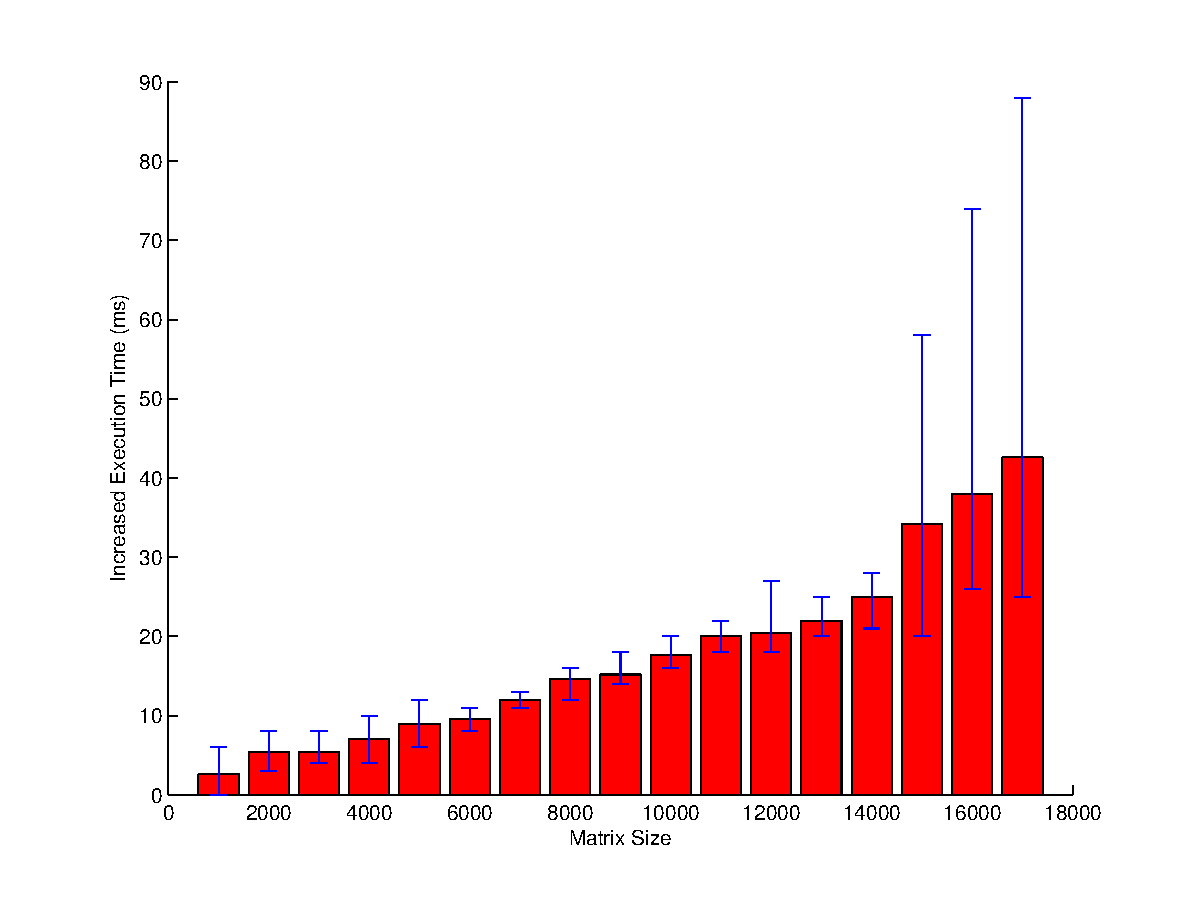
\includegraphics[width=0.5\textwidth]{tolerance}
\caption{Average Extra Execution Time When the accuracy increase Performance Comparision}
\label{fig:tolerance}
\end{figure}
Figure \ref{fig:tolerance} shows the average increased execution time when the accuracy of singular values goes up a higher level on different matrix size.
In other word, it shows the average increased execution time when the error tolerance becomes smaller from $10^{-x}$ to $10^{-(x+1)}$.
From the figure, we can see that when matrix size is smaller than 12000, the additional execution time is only less than $20 ms$ when the error tolerance rises a level.
When the matrix size is larger than 15000, the additional execution time is a little higher about $40 ms$ per level.

\subsection{Pthread CUDA Result}
\subsubsection{Load Balance}
\begin{figure}[hbpt]
\centering
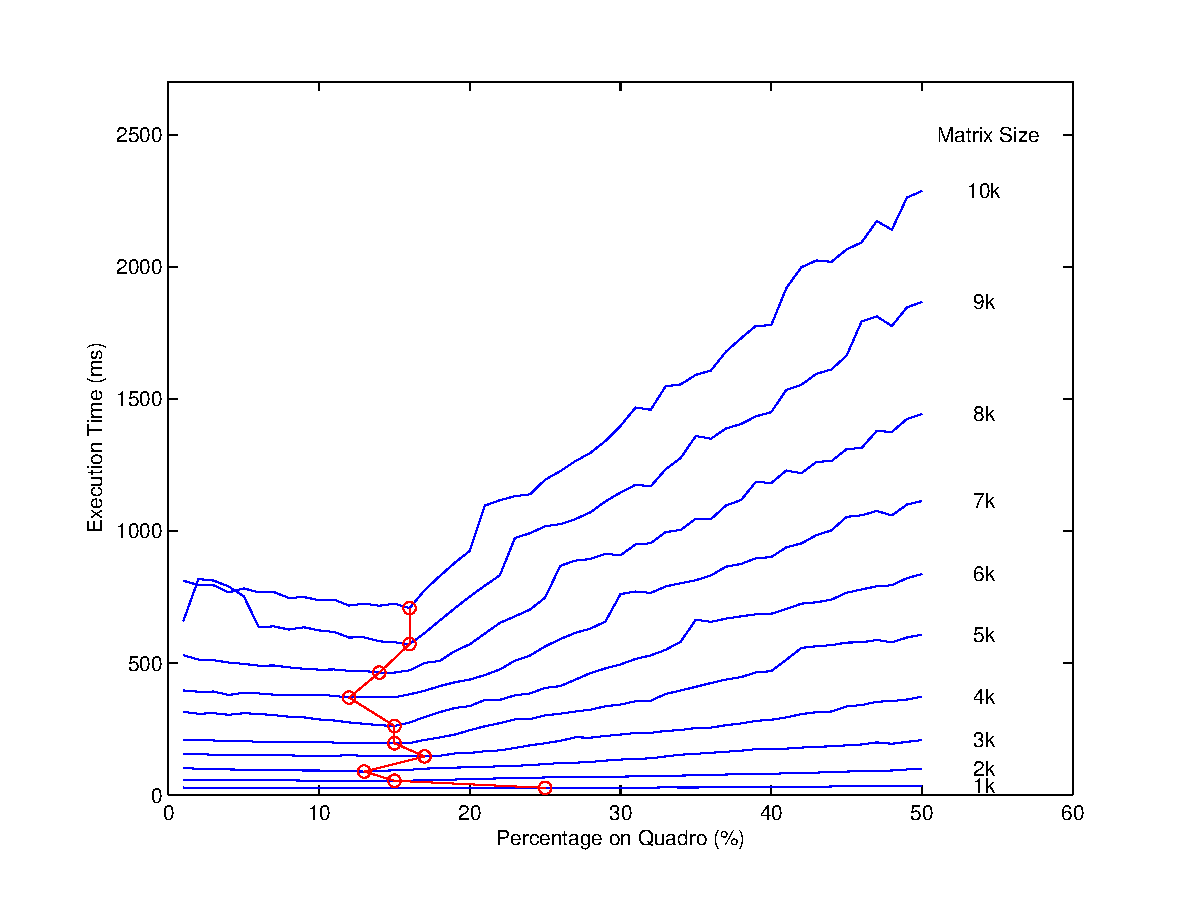
\includegraphics[width=0.5\textwidth]{pthread}
\caption{Load Balance on GeForce and Quadro}
\label{fig:pthread}
\end{figure}
Figure \ref{fig:pthread} shows the total execution time with different load balance on a system of two different GPUs.
The horizontal axis represents the percentage of work on Quadro 600.
The other percentage of work will be moved to GeForce 750 Ti obviously.
The red points represent the minimum values in the blue curves.
The blue curves can be separated into two parts by red points.
The left ones are dominated by GeForce 750 Ti, while the right ones are contributed by Quadro 600.
Since Quadro 600 has a worse performance than GeForce 750 Ti, less work is allocated on it.
When around 15\% of work is executed on Quadro 600, and 85\% of that is processed on GeForce 750 Ti,
the total performance of the system will be better than others.

\textbf{A table to shows the Huge Size Result. This part do not compare to other results.} 

\begin{table}[h]
\caption{Performance of Huge Size Matrix}
\centering
\begin{tabular}{|c|c|c|c|}
\hline
Matrix Size & GeForce & Quadro & GeForce + Quadro \\ \hline
 10K*10K    &   0.8s  &  4.6s  &   0.7s (85\%) / 0.7s (15\%) \\ \hline
 20K*20K    &   2.9s  &   18s  &   2.6s (85\%) / 2.7s (15\%) \\ \hline
 30K*30K    &   6.7s  &   37s  &   5.9s (85\%) / 5.6s (15\%) \\ \hline
 40K*40K    &    12s  &   63s  &    10s (85\%) / 9.5s (15\%) \\ \hline
 50K*50K    &    19s  &   96s  &    16s (84\%) /  15s (16\%) \\ \hline
 80K*80K    &    50s  &  238s  &    43s (84\%) /  40s (16\%) \\ \hline
 100K*100K  &    84s  &  393s  &    71s (83\%) /  67s (17\%) \\ \hline
 120K*120K  &   134s  &     -  &   113s (82\%) / 102s (18\%) \\ \hline
 150K*150K  &   245s  &     -  &   203s (81\%) / 194s (19\%) \\ \hline
 180K*180K  &   412s  &     -  &   340s (80\%) / 337s (20\%) \\ \hline
 200K*200K  &   555s  &     -  &   -  \\ \hline
\end{tabular}
\label{tab:hresult}
\end{table}

\begin{table}[h]
\caption{Performance of Huge Size Matrix with double floating-point on Tesla}
\centering
\begin{tabular}{|c|c|c|}
\hline
Matrix Size &  Tesla  & Tesla (50\%) + Tesls (50\%) \\ \hline
 10K*10K    &   s  &  1.2s / 0.6s \\ \hline
 20K*20K    &   s  &  4.9s / 3.6s \\ \hline
 30K*30K    &   s  &   12s / 9.3s \\ \hline
 40K*40K    &   s  &   21s /  18s \\ \hline
 50K*50K    &   s  &   41s /  36s \\ \hline
% 60K*60K    &   s  &   55s /  47s \\ \hline
% 70K*70K    &   s  &   73s /  59s \\ \hline
 80K*80K    &   s  &  103s /  81s \\ \hline
% 90K*90K    &   s  &  145s / 115s \\ \hline
 100K*100K  &   s  &  190s / 154s \\ \hline
% 110K*110K  &   s  &  231s / 178s \\ \hline
 120K*120K  &   s  &  286s / 243s \\ \hline
% 130K*130K  &   s  &  286s / 217s \\ \hline
% 140K*140K  &   s  &  359s / 292s \\ \hline
 150K*150K  &   s  &  469s / 399s \\ \hline
% 160K*160K  &   s  &  473s / 378s \\ \hline
% 170K*170K  &   s  &  491s / 379s \\ \hline
 180K*180K  &   s  &     -  \\ \hline
% 190K*190K  &   s  &     -  \\ \hline
 200K*200K  &   s  &     -  \\ \hline
\end{tabular}
\label{tab:hresult}
\end{table}

